% =====================================================================
%  CHƯƠNG 5. TRIỂN KHAI MÔ HÌNH TRÊN THIẾT BỊ BIÊN
%  Nguồn số: runs/pi_hailo_measured_2026-08-24.md, runs/pi_camera_measured_2026-08-27.md,
%            runs/flight_val_hef_2026-08-27.md, runs/retrain_coco_2026-08-27.md
% =====================================================================
\chapter{Triển khai mô hình trên thiết bị biên}
\label{chap:trienkhai}

Một mô hình chính xác trên máy tính huấn luyện chưa chắc dùng được trên máy bay. Chương này trình bày quá trình đưa SteadyDet-N lên Raspberry Pi~5 gắn NPU Hailo-8L: chuẩn bị mô hình cho trình biên dịch, lượng tử hoá INT8, đo độ chính xác sau lượng tử hoá trên hai miền dữ liệu, đo tốc độ và độ trễ đầu-cuối với camera thật. Mọi con số trong chương đều được đo trực tiếp trên phần cứng đích.

\section{Nền tảng phần cứng}

Máy tính đồng hành là Raspberry Pi~5 chạy Debian~12. NPU Hailo-8L gắn qua khe M.2 và đường PCIe; trong cấu hình đo, liên kết hoạt động ở tốc độ Gen2 x1 (5\,GT/s). Camera là Logitech C270 HD cắm cổng USB, dùng định dạng nén MJPG. Bộ điều khiển bay Pixhawk~6C nối với Pi qua USB. Phần suy luận chạy trên NPU; các phần còn lại (đọc camera, tiền xử lý, giải mã, NMS, theo vết, điều khiển, bảng giám sát web) chạy trên CPU của Pi.

\begin{figure}[H]
\centering
\resizebox{\textwidth}{!}{% Quy trình đưa mô hình từ PyTorch lên NPU Hailo-8L
\begin{tikzpicture}[
  font=\footnotesize, >={Stealth[length=2mm]},
  st/.style={draw=black!60, rounded corners=2pt, align=center, minimum height=11mm, text width=2.45cm, inner sep=2pt, fill=white},
  pc/.style={st, fill=black!5},
  hw/.style={st, fill=xanh!14},
  note/.style={font=\scriptsize, text=black!70, align=center, text width=2.5cm}
]
\node[pc] (a) {Checkpoint PyTorch\\(FP32, bỏ self-attention)};
\node[pc, right=6mm of a] (b) {Xuất ONNX\\opset 11, kích thước tĩnh};
\node[pc, right=6mm of b] (c) {DFC: phân tích đồ thị\\4 bản đồ đầu ra};
\node[pc, right=6mm of c] (d) {DFC: lượng tử hoá INT8\\64 ảnh hiệu chuẩn (tập huấn luyện)};
\node[pc, right=6mm of d] (e) {DFC: biên dịch\\$\rightarrow$ tệp HEF (4 context)};
\foreach \x/\y in {a/b,b/c,c/d,d/e} \draw[->] (\x) -- (\y);
\node[note, below=1mm of a] {tinh chỉnh 20 epoch\\có COCO-person};
\node[note, below=1mm of b] {gộp BN vào Conv,\\\texttt{dynamo=False}};

\node[font=\footnotesize\bfseries, anchor=west] at ($(a.north west)+(0,0.35)$) {Máy tính x86 (biên dịch một lần)};

\node[hw, below=3.0cm of b] (f) {Camera C270\\khung $640\times480$};
\node[hw, right=6mm of f] (g) {Tiền xử lý CPU\\letterbox 640};
\node[hw, right=6mm of g] (h) {Suy luận INT8\\NPU Hailo-8L};
\node[hw, right=6mm of h] (i) {Giải mã + NMS\\CPU (NumPy)};
\foreach \x/\y in {f/g,g/h,h/i} \draw[->] (\x) -- (\y);
\draw[->, dashed] (e.south) -- ++(0,-0.75) -| (h.north);
\node[font=\footnotesize\bfseries, anchor=west] at ($(f.north west)+(0,0.35)$) {Raspberry Pi~5 trên máy bay (mỗi khung hình)};
\end{tikzpicture}
}
\caption{Quy trình đưa mô hình lên NPU: biên dịch một lần trên máy tính x86 (trên) và chuỗi xử lý mỗi khung hình trên Raspberry Pi~5 (dưới)}
\label{fig:quytrinhtrienkhai}
\end{figure}

\section{Chuẩn bị mô hình cho trình biên dịch}

\subsection{Loại bỏ khối self-attention}

Trình biên dịch Hailo DFC không hỗ trợ các phép biến đổi hình dạng tensor mà khối self-attention theo cửa sổ sử dụng. Đề tài xử lý bằng cách tạo một cấu hình SteadyDet-N không có khối này (thuần tích chập, 0,875 triệu tham số) và tinh chỉnh 20 epoch từ checkpoint của nhánh triển khai với learning rate $10^{-3}$. Việc kiểm tra tệp ONNX sau khi xuất xác nhận đồ thị không còn các phép toán MatMul, Softmax hay ReduceMean. Việc chuyển đổi này có ảnh hưởng tới độ chính xác, được định lượng ở mục~\ref{sec:chonhef}.

\subsection{Một lỗi cấu hình và cách phát hiện}

Lần tinh chỉnh đầu tiên cho kết quả kém bất thường trên dữ liệu bay thật: F1 của bản FP32 chỉ đạt 0,768 so với 0,882 của checkpoint trước khi tinh chỉnh. Khi phân tích nhật ký huấn luyện, nhóm nhận thấy toàn bộ mẫu dương đều rơi vào hai mức $P_2$ và $P_3$ (số mẫu dương ở $P_4$ và $P_5$ bằng 0), tức mô hình không hề thấy người kích thước lớn trong suốt quá trình tinh chỉnh. Nguyên nhân là tệp cấu hình đặt epoch bắt đầu trộn COCO-person bằng 100 trong khi toàn bộ quá trình chỉ có 20 epoch, nên dữ liệu người cự ly gần chưa bao giờ được bật. Sau khi sửa để trộn COCO ngay từ epoch đầu, nhật ký xác nhận có mẫu dương ở cả $P_4$ và $P_5$, và F1 trên dữ liệu bay thật tăng từ 0,768 lên 0,836, lấy lại 60\% khoảng cách. Phần chênh lệch còn lại (0,046) là cái giá của việc bỏ khối self-attention trên miền bay thấp. Bài học rút ra là: kiểm tra phân bố mẫu dương theo mức là một cách rẻ để phát hiện dữ liệu huấn luyện không đúng như ý định.

\subsection{Xuất ONNX}

Mô hình được gộp các lớp batch norm vào tích chập, xuất ONNX với kích thước đầu vào tĩnh $640\times640$ và opset 11. Đầu ra là bốn bản đồ dự đoán thô; phần giải mã theo phương trình~(\ref{eq:decode}) và NMS chạy trên CPU. Nhóm gặp một lỗi khi xuất: từ PyTorch 2.6, hàm xuất ONNX mặc định dùng bộ xuất mới, bộ này bỏ thuộc tính \texttt{kernel\_shape} của nút tích chập (vẫn hợp lệ theo chuẩn ONNX) nhưng trình phân tích của Hailo lại đọc trực tiếp thuộc tính này và dừng với lỗi chỉ số. Buộc dùng bộ xuất cũ (\texttt{dynamo=False}) cho tệp opset 11 với đủ 82/82 nút tích chập có thuộc tính này. Để chắc chắn tệp ONNX tương đương PyTorch, nhóm chạy toàn bộ phép quét ngưỡng trên dữ liệu bay thật bằng cả hai: F1 đạt 0,831 (ONNX) so với 0,836 (PyTorch), số dự đoán đúng giống hệt ở mọi ngưỡng.

\section{Lượng tử hoá và biên dịch}

Tệp ONNX được DFC lượng tử hoá INT8 với mức tối ưu 2 và biên dịch thành tệp HEF gồm 4 context. Tập ảnh hiệu chuẩn được lấy từ \textit{tập huấn luyện}, trộn đúng tỷ lệ dùng khi huấn luyện (75\% VisDrone, 25\% COCO-person). Tập flight\_val không được dùng để hiệu chuẩn vì đó là tập đánh giá. Nhóm biên dịch hai phiên bản: một với 64 ảnh hiệu chuẩn và một với 512 ảnh.

\section{Độ chính xác sau lượng tử hoá}
\label{sec:int8}

\subsection{Chọn tệp HEF triển khai}
\label{sec:chonhef}

Ba tệp HEF được đo trên Pi, cùng 92 khung bay thật và cùng một đường giải mã (Bảng~\ref{tab:hef}).

\begin{table}[H]
\centering
\caption{So sánh các tệp HEF trên 92 khung bay thật; mỗi tệp dùng ngưỡng tin cậy cho F1 cao nhất của chính nó}
\label{tab:hef}
\small
\renewcommand{\arraystretch}{1.15}
\begin{tabularx}{\textwidth}{@{}>{\raggedright\arraybackslash}Xcccccc@{}}
\toprule
\textbf{Tệp HEF} & \textbf{Ảnh hiệu chuẩn} & \textbf{Ngưỡng} & \textbf{F1} & \textbf{Độ phủ} & \textbf{Độ chuẩn xác} & \textbf{FPS}\\
\midrule
\textbf{Có COCO, 64 ảnh (triển khai)} & 64 & 0,25 & \textbf{0,880} & \textbf{0,837} & 0,928 & 56,9\\
Có COCO, 512 ảnh & 512 & 0,25 & 0,812 & 0,750 & 0,885 & 62,9\\
Bản trước (chưa trộn COCO) & -- & 0,30 & 0,745 & 0,620 & 0,934 & 63,7\\
\bottomrule
\end{tabularx}
\end{table}

Tệp dùng 64 ảnh hiệu chuẩn cho F1 cao nhất và recall 0,837, tức bắt được người ở 84\% số khung thay vì 62\% như bản trước. Nó chậm hơn khoảng 2\,ms mỗi khung (17,6\,ms so với 15,7\,ms) nhưng vẫn dư xa ngân sách 33,3\,ms, nên được chọn để triển khai. Một kết quả trái trực giác: 512 ảnh hiệu chuẩn cho kết quả kém hơn 64 ảnh, dù trình biên dịch khuyến nghị nhiều ảnh hơn. Nhóm chưa xác định được cơ chế; bài học vận hành là phải đo trên dữ liệu miền triển khai thay vì dựa vào khuyến nghị chung.

\subsection{Tổn thất INT8 phụ thuộc kích thước đối tượng}

Để đo đúng tổn thất do lượng tử hoá, dự đoán FP32 (trên GPU) và INT8 (trên NPU) của cùng một mô hình được xuất ra cùng một định dạng và chấm bằng cùng một hàm, trên cả hai miền dữ liệu (Bảng~\ref{tab:int8}, Hình~\ref{fig:int8}).

\begin{table}[H]
\centering
\caption{Độ chính xác FP32 và INT8 của mô hình triển khai, cùng một chương trình chấm điểm}
\label{tab:int8}
\small
\renewcommand{\arraystretch}{1.15}
\begin{tabular}{@{}lccc|ccc@{}}
\toprule
 & \multicolumn{3}{c|}{\textbf{VisDrone-val (548 ảnh, người rất nhỏ)}} & \multicolumn{3}{c}{\textbf{Bay thật $\approx$6\,m (92 khung)}}\\
\textbf{Chỉ số} & \textbf{FP32} & \textbf{INT8} & \textbf{Thay đổi} & \textbf{FP32} & \textbf{INT8} & \textbf{Thay đổi}\\
\midrule
AP@[.50:.95] & 0,1775 & 0,1584 & $-$10,8\% & 0,4356 & 0,4349 & $-$0,2\%\\
AP@0,50 & 0,4946 & 0,4625 & $-$6,5\% & 0,8822 & \textbf{0,9171} & +4,0\%\\
AP@0,75 & 0,0742 & 0,0555 & $-$25,2\% & 0,2561 & 0,2552 & $-$0,4\%\\
AR@100 & 0,3041 & 0,2869 & $-$5,7\% & 0,5489 & 0,5337 & $-$2,8\%\\
\bottomrule
\end{tabular}
\end{table}

\begin{figure}[H]
\centering
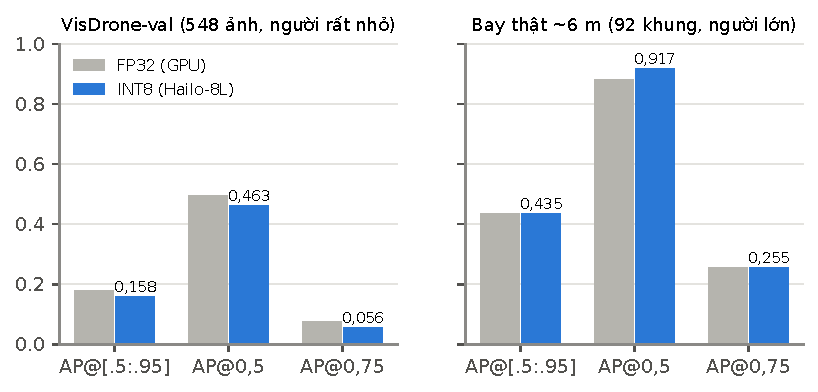
\includegraphics[width=\textwidth]{int8.pdf}
\caption{Độ chính xác FP32 và INT8 trên hai miền dữ liệu. Trên người rất nhỏ, INT8 làm hộp kém khít (AP@0,75 giảm 25\%); trên người ở độ cao bay thực tế, hai bản gần như trùng nhau}
\label{fig:int8}
\end{figure}

Trên VisDrone-val, AP@0,5 chỉ giảm 6,5\% còn AP@0,75 giảm 25,2\%: lượng tử hoá không làm mất đối tượng mà làm hộp kém khít. Điều này phù hợp với phân tích ở Chương~\ref{chap:lythuyet}: điểm tin cậy chịu được lượng tử hoá, còn toạ độ hộp mất độ phân giải, và với người chỉ vài điểm ảnh, sai lệch nhỏ đó đủ làm IoU tụt dưới 0,75. Trên dữ liệu bay thật, người chiếm hàng nghìn điểm ảnh nên cùng sai lệch gần như không đáng kể: hai bản khác nhau không quá 0,035 ở mọi chỉ số, nằm trong sai số lấy mẫu của 92 khung. Phát biểu chính xác là: \textbf{INT8 tốn khoảng 6,5\% AP@0,5 với người rất nhỏ và gần như không tốn gì với người ở độ cao bay 3--6\,m}. Kết quả này cũng điều chỉnh một kết luận bi quan trước đó của nhóm, khi lượng tử hoá sau huấn luyện đơn giản trên ONNX từng làm AP sụp từ 0,18 xuống 0,009; hiệu chuẩn theo từng lớp của DFC tốt hơn nhiều.

\textbf{Chỉ tiêu độ chính xác của đề tài.} Mô hình đang chạy trên máy bay đạt AP@0,5 = 0,917 trên dữ liệu bay thật, vượt chỉ tiêu 70\% trong thuyết minh. Con số này là của đúng mô hình INT8 trên NPU chứ không phải của một checkpoint trên máy tính huấn luyện. Lưu ý không so sánh trực tiếp con số 0,917 với 0,7613 ở Bảng~\ref{tab:baythat}: hai con số thuộc hai checkpoint khác nhau và được tính bằng hai đường giải mã khác nhau; Bảng~\ref{tab:baythat} dùng để so sánh \textit{dữ liệu và cách xử lý rung}, còn Bảng~\ref{tab:int8} dùng để đánh giá \textit{hệ thống triển khai}.

\subsection{Chọn ngưỡng tin cậy vận hành}

Ngưỡng tin cậy quyết định trực tiếp hành vi trên máy bay: quá cao thì bỏ sót người, quá thấp thì bám nhầm vào hộp sai. Với bản HEF trước, ngưỡng 0,40 chỉ bắt được người ở 19,6\% số khung, còn ngưỡng 0,20 sinh trung bình 1,30 hộp sai mỗi khung, khớp đúng hiện tượng người dùng quan sát được khi thử (``chĩa vào người không thấy gì'' và ``hạ ngưỡng thì nhiễu''). Hình~\ref{fig:nguong} là kết quả quét ngưỡng cho bản HEF triển khai: F1 đạt cực đại 0,880 tại ngưỡng 0,25 và giảm còn 0,551 ở ngưỡng 0,40. Ngưỡng tối ưu thay đổi theo từng tệp HEF (bản trước là 0,30), nên mỗi lần đổi mô hình phải quét lại.

\begin{figure}[H]
\centering
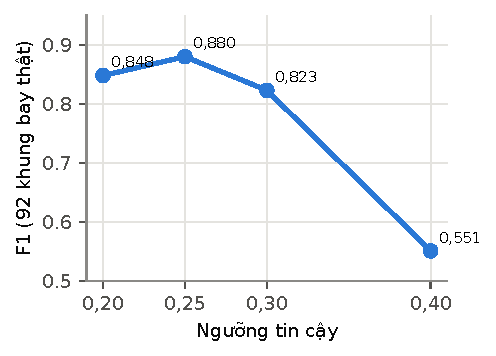
\includegraphics[width=0.5\textwidth]{nguong_conf.pdf}
\caption{F1 của mô hình triển khai theo ngưỡng tin cậy trên 92 khung bay thật}
\label{fig:nguong}
\end{figure}

\section{Tốc độ suy luận trên NPU}

\subsection{Tốc độ theo từng khung và theo lô}

Tốc độ được đo bằng công cụ chuẩn \texttt{hailortcli benchmark} của Hailo và kiểm tra chéo bằng lời gọi đồng bộ từ Python; hai cách cho kết quả khớp nhau. Với batch size 1, SteadyDet-N đạt \textbf{112,55 FPS (8,40\,ms)} ở $320\times320$ và \textbf{63,66 FPS (15,26\,ms)} ở $640\times640$. Bản HEF triển khai đạt 56,9 FPS, độ trễ suy luận trung vị 17,32\,ms và p99 17,52\,ms đo trong lượt đánh giá 548 ảnh.

\begin{table}[H]
\centering
\caption{Thông lượng và độ trễ theo batch size trên Hailo-8L (mô hình $320\times320$)}
\label{tab:batch}
\small
\renewcommand{\arraystretch}{1.15}
\begin{tabular}{@{}ccc@{}}
\toprule
\textbf{Kích thước lô} & \textbf{Thông lượng (FPS)} & \textbf{Độ trễ phần cứng (ms)}\\
\midrule
1 & 112,55 & 8,40\\
4 & 188,78 & 17,05\\
8 & 214,63 & 28,35\\
16 & 231,82 & 50,48\\
\bottomrule
\end{tabular}
\end{table}

Bảng~\ref{tab:batch} cho thấy tăng batch size làm tăng thông lượng nhưng cũng làm tăng độ trễ mỗi khung. Hệ thống bám người dùng lô 1 vì hai lý do: độ trễ phần cứng tăng từ 8,40 lên 17,05\,ms ở lô 4, và với camera 30 khung/giây, riêng việc chờ gom đủ 4 khung đã mất thêm 133\,ms, một độ trễ mà vòng điều khiển bám người không chấp nhận được. Thông lượng và độ trễ là hai đại lượng khác nhau và không được nhầm lẫn khi báo cáo.

\subsection{So sánh với YOLO26-n trên cùng một chip}

Để kiểm tra luận điểm hiệu quả tính toán trên phần cứng thật, đề tài biên dịch YOLO26-n (chính checkpoint dùng trong Bảng~\ref{tab:sosanh}) bằng đúng cùng lệnh và tham số, cắt đồ thị tại các tích chập đầu ra để phần giải mã và NMS của cả hai mô hình đều chạy trên CPU, rồi đo trên cùng Pi.

\begin{table}[H]
\centering
\caption{SteadyDet-N và YOLO26-n trên cùng Hailo-8L, ảnh $640\times640$, lô 1}
\label{tab:yolo26hailo}
\small
\renewcommand{\arraystretch}{1.15}
\begin{tabular}{@{}lccccc@{}}
\toprule
\textbf{Mô hình} & \textbf{Tham số (M)} & \textbf{GFLOPs} & \textbf{Số context} & \textbf{FPS} & \textbf{Độ trễ (ms)}\\
\midrule
\textbf{SteadyDet-N} & \textbf{1,17} & \textbf{4,6} & \textbf{4} & \textbf{63,66} & \textbf{15,26}\\
YOLO26-n & 2,38 & 5,2 & 6 & 37,46 & 24,79\\
\bottomrule
\end{tabular}
\end{table}

SteadyDet-N \textbf{nhanh hơn 1,70 lần} với 49\% số tham số và 88\% chi phí tính toán (Bảng~\ref{tab:yolo26hailo}, Hình~\ref{fig:hailo}). Mức chênh lệch tốc độ lớn hơn nhiều so với mức chênh lệch GFLOPs; cơ chế nằm ở số context: SteadyDet-N vừa 4 context còn YOLO26-n cần 6, và mỗi lần chuyển context NPU phải nạp lại trọng số qua PCIe. Trên loại chip này, giảm kích thước mô hình để giảm số context quan trọng không kém giảm số phép tính. Hai tệp HEF trong phép so sánh này được hiệu chuẩn bằng ảnh kiểm định, nên chỉ dùng để so tốc độ, không dùng để lấy độ chính xác. Số tham số và GFLOPs của YOLO26-n ở đây được tính trên đồ thị đã xuất để biên dịch, nên khác một chút so với Bảng~\ref{tab:sosanh}.

\begin{figure}[H]
\centering
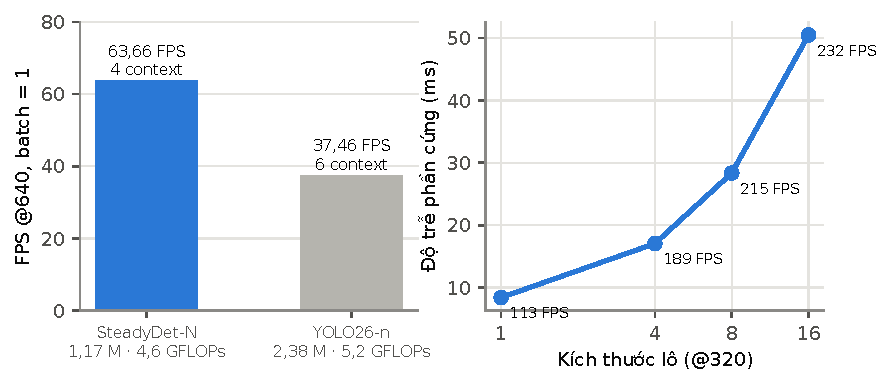
\includegraphics[width=\textwidth]{hailo.pdf}
\caption{Trái: tốc độ SteadyDet-N và YOLO26-n trên cùng Hailo-8L. Phải: độ trễ phần cứng tăng theo batch size dù thông lượng tăng}
\label{fig:hailo}
\end{figure}

\section{Độ trễ đầu-cuối với camera thật}
\label{sec:e2e}

\subsection{Hai lỗi phía camera làm hệ thống kẹt ở 15 khung hình/giây}

Lần đo đầu tiên với camera thật chỉ đạt 15,4 khung hình/giây, trong khi NPU mới dùng khoảng 17,8\,ms trong ngân sách 33,3\,ms. Đo tách riêng từng chặng cho thấy nút cổ chai không nằm ở mô hình mà ở camera, do hai lỗi độc lập nhân với nhau (Hình~\ref{fig:camera}):
\begin{enumerate}
\item \textbf{Bộ đệm camera bằng 1.} Tham số \texttt{CAP\_PROP\_BUFFERSIZE = 1} vốn được đặt để luôn lấy khung mới nhất, nhưng khi ứng dụng đang giữ bộ đệm duy nhất, trình điều khiển không có chỗ ghi khung kế tiếp nên bỏ luôn khung đó: 30 khung/giây thành đúng 15,0. Tăng lên 2 cho 30,0 khung/giây, còn độ cũ của khung đo được chỉ trung vị 15,7\,ms, bằng nửa chu kỳ khung như lý thuyết.
\item \textbf{Tự phơi sáng tự hạ tốc độ khung.} Khi thiếu sáng, firmware của camera kéo dài thời gian phơi sáng quá 1/30\,s và tự giảm tốc độ khung (đo được 24,9 khung/giây ở thời gian phơi sáng 1/25\,s). Cờ UVC dùng để cấm hành vi này bị firmware bỏ qua. Đề tài giải quyết bằng cách khoá phơi sáng thủ công và tự viết bộ điều chỉnh độ sáng bằng phần mềm (SoftAE) có trần thời gian phơi sáng cứng: đo độ sáng trung bình mỗi khung rồi điều chỉnh thời gian phơi sáng và độ khuếch đại. Kết quả: độ sáng bám giá trị đặt, tốc độ khung giữ 30,1.
\end{enumerate}
Sau khi sửa cả hai, tốc độ tăng từ 11,1 lên 30,0 khung hình/giây mà không thay đổi dòng nào của mô hình. Tần số lưới điện của camera cũng được đặt về 50\,Hz theo điện lưới Việt Nam để tránh sọc nhấp nháy dưới đèn huỳnh quang.

\begin{figure}[H]
\centering
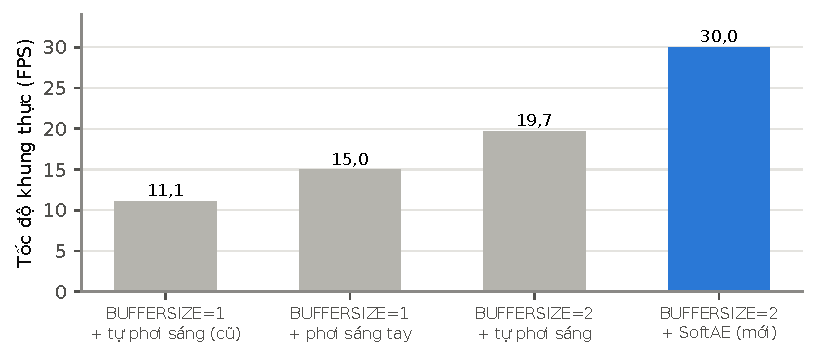
\includegraphics[width=0.9\textwidth]{camera_fps.pdf}
\caption{Tốc độ khung thực tế của chuỗi xử lý với bốn cấu hình camera}
\label{fig:camera}
\end{figure}

\subsection{Phân tích độ trễ từng chặng}

Chuỗi xử lý được đo liên tục trong 2 phút với camera thật ở $640\times640$ (3.594 khung). Bảng~\ref{tab:e2e} và Hình~\ref{fig:dotre} trình bày kết quả.

\begin{table}[H]
\centering
\caption{Độ trễ từng chặng của chuỗi xử lý trên Raspberry Pi~5 + Hailo-8L (ms), 3.594 khung}
\label{tab:e2e}
\small
\renewcommand{\arraystretch}{1.15}
\begin{tabular}{@{}lccccc@{}}
\toprule
\textbf{Chặng} & \textbf{Trung bình} & \textbf{p50} & \textbf{p95} & \textbf{p99} & \textbf{Lớn nhất}\\
\midrule
Chờ và đọc khung camera & 13,85 & 12,47 & 16,52 & 16,91 & 226,64\\
Tiền xử lý (letterbox, đổi kênh màu) & 0,98 & 0,99 & 1,02 & 1,04 & 1,67\\
Suy luận trên NPU & 17,73 & 17,72 & 17,83 & 17,89 & 18,09\\
Giải mã + NMS & 0,84 & 0,84 & 0,87 & 0,88 & 7,57\\
\midrule
\textbf{Tổng} & \textbf{33,39} & \textbf{32,04} & \textbf{36,08} & \textbf{36,15} & 246,76\\
\bottomrule
\end{tabular}
\end{table}

\begin{figure}[H]
\centering
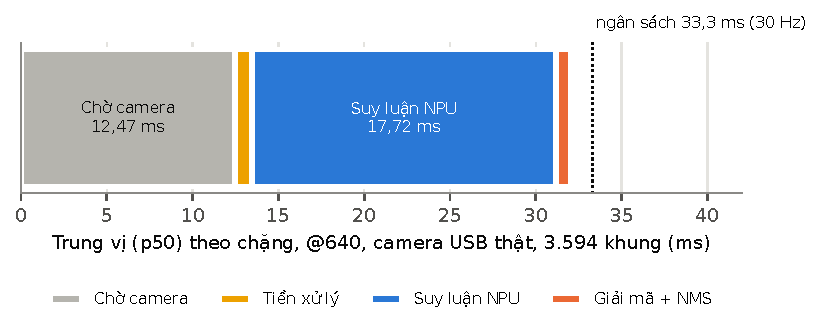
\includegraphics[width=\textwidth]{do_tre.pdf}
\caption{Phân bổ độ trễ trung vị theo chặng so với ngân sách 33,3\,ms của vòng lặp 30\,Hz}
\label{fig:dotre}
\end{figure}

Ba chặng tính toán (tiền xử lý, suy luận, giải mã) cộng lại chỉ 19,55\,ms trong ngân sách 33,3\,ms, tức hệ số sử dụng 59\%; phần còn lại là thời gian chờ camera. Hệ thống vì thế \textbf{bị giới hạn bởi camera chứ không bởi mô hình}: camera C270 tối đa 30 khung/giây, và muốn nhanh hơn thì phải đổi camera. Tốc độ khung giữ 29,9 ở phút đầu và 30,0 ở phút cuối, nhiệt độ SoC 48,5\,°C, cờ giảm xung nhiệt bằng 0 trong suốt thời gian đo. Khoảng dao động của chặng suy luận rất hẹp (p50 17,72\,ms, p99 17,89\,ms), điều quan trọng với bộ điều khiển vì nó phụ thuộc vào khung chậm nhất chứ không phải khung trung bình. Giá trị lớn nhất (246,76\,ms) chỉ là các khung cá biệt ở chặng camera, không ảnh hưởng tới p99.

Phép đo đầu-cuối này được thực hiện với bản HEF $640\times640$ cùng kiến trúc trước khi tệp triển khai cuối cùng được biên dịch; bản triển khai có độ trễ suy luận trung vị 17,32\,ms, tương đương, nên kết luận về ngân sách thời gian vẫn giữ nguyên.

\section{Kết luận chương}

SteadyDet-N đã được đưa lên Raspberry Pi~5 + Hailo-8L thành công. Mô hình INT8 đạt AP@0,5 = 0,917 và F1 = 0,880 trên dữ liệu bay thật ở ngưỡng tin cậy 0,25; tổn thất lượng tử hoá đáng kể với người rất nhỏ nhưng không đáng kể với người ở độ cao bay thực tế. Trên NPU, mô hình chạy nhanh hơn YOLO26-n 1,70 lần nhờ cần ít context hơn. Toàn bộ chuỗi camera -- suy luận -- hậu xử lý đạt 30 khung hình/giây ổn định, với các chặng tính toán chỉ chiếm 59\% ngân sách thời gian. Hai lỗi phía camera được phát hiện và sửa nhờ đo từng chặng, cho thấy tầm quan trọng của việc đo trước khi tối ưu.
